\begin{figure}[H]
\centering
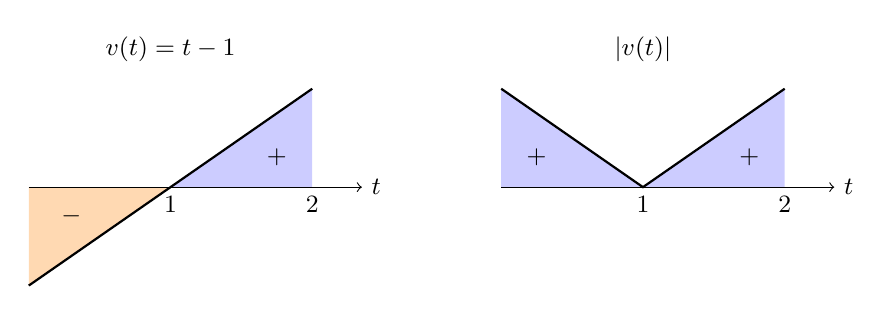
\begin{tikzpicture}[x=1.8cm,y=1.25cm,font=\small]
\begin{scope}
\fill[orange!30] (0,0)--(0,-1)--(1,0)--cycle;
\fill[blue!20] (1,0)--(2,1)--(2,0)--cycle;
\draw[->] (0,0)--(2.35,0) node[right] {$t$};
\draw[thick] (0,-1)--(2,1);
\node at (1,1.4) {$v(t)=t-1$};
\node at (.3,-.3) {$-$};\node at (1.75,.3) {$+$};
\node[below] at (1,0) {$1$};\node[below] at (2,0) {$2$};
\end{scope}
\begin{scope}[xshift=6cm]
\fill[blue!20] (0,0)--(0,1)--(1,0)--(2,1)--(2,0)--cycle;
\draw[->] (0,0)--(2.35,0) node[right] {$t$};
\draw[thick] (0,1)--(1,0)--(2,1);
\node at (1,1.4) {$|v(t)|$};
\node at (.25,.3) {$+$};\node at (1.75,.3) {$+$};
\node[below] at (1,0) {$1$};\node[below] at (2,0) {$2$};
\end{scope}
\end{tikzpicture}
\caption{Displacement adds signed contributions (left), giving zero here.
Distance adds their magnitudes (right), giving one metre.}
\label{fig:velocity-distance}
\end{figure}
